\documentclass{article}
\newcommand{\mydate}{September 24, 2025}
\newcommand{\mytitle}{QM HW4}
\title{\textbf{\mytitle}}
\author{Jiete XUE}
\date{\mydate}
\usepackage{fancyhdr}
\pagestyle{fancy}
\fancyhf{}
\fancyhead[C]{\mytitle }
\fancyhead[R]{Jiete Xue}
\fancyhead[L]{\mydate}
\fancyfoot[C]{\thepage}
\usepackage{amsthm}
\usepackage{amsmath}
\usepackage{amssymb}
\usepackage{physics}
\usepackage{tikz}

%% 右矢
%\ket{\psi}          % 输出:|ψ⟩
%\ket{\psi(t)}       % 输出:|ψ(t)⟩
%
%% 左矢
%\bra{\phi}          % 输出:⟨φ|
%
%% 期望值
%\expval{\hat{A}}    % 输出:⟨Â⟩
%\expval{\hat{A}}{\psi}  % 输出:⟨ψ|Â|ψ⟩
%
%% 对易子
%\comm{\hat{A}}{\hat{B}}  % 输出:[Â, B̂]
\newtheoremstyle{1}{}{}{}{}{\bfseries}{}{\newline}{}
\theoremstyle{1}
\newtheorem{problem}{Problem}
\usepackage{chngcntr}
\counterwithin{equation}{problem}
\newcommand{\pa}{\partial}
\newcommand{\rn}[1]{\romannumeral #1\relax}
\newcommand{\Rn}[1]{\expandafter\@slowromancap\romannumeral#1@}

\begin{document}
\maketitle
\begin{problem}[Probability current]
    By definition
    \begin{equation}\label{1.1}
        \frac{\pa \rho}{\pa t}=\frac{\pa \psi^*}{\pa t}\psi+\psi^*\frac{\pa\psi}{\pa t}.
    \end{equation}
    By Schrödinger equation,
    \begin{equation}
        \frac{\pa \psi}{\pa t}=\frac{i\hbar}{2m}\nabla^2\psi-\frac{iV}{\hbar}\psi.
    \end{equation}
    \begin{equation}
        \frac{\pa \psi^*}{\pa t}=-\frac{i\hbar}{2m}\nabla^2\psi^*+\frac{iV}{\hbar}\psi^*.\footnote{$V^*=V$.}
    \end{equation}
    Plug in \eqref{1.1},
    \begin{equation}
        \frac{\pa \rho}{\pa t}=\frac{i\hbar}{2m}\left[\psi^*\nabla^2\psi-\psi\nabla^2\psi^*\right]=\frac{i\hbar}{2m}\nabla\cdot\left[\psi^*\nabla\psi-\psi\nabla\psi^*\right].
    \end{equation}
    Let 
    \begin{equation}
        \boxed{\vec{j}=-\frac{i\hbar}{2m}\left[\psi^*\nabla\psi-\psi\nabla\psi^*\right].}
    \end{equation}
    Then,
    \begin{equation}
        \frac{\pa \rho}{\pa t}+\nabla\cdot\vec{j}=0.
    \end{equation}
\end{problem}
\begin{problem}[time-evolution]
    (1) \begin{equation}
        \frac{\dd{\bar{O}}}{\dd{t}}=\frac{\pa }{\pa t}\bra{\psi}O\ket{\psi}+\bra{\psi}O\frac{\pa}{\pa t}\ket{\psi}.
    \end{equation}
    The Schrödinger equation in bra-ket form is
    \begin{equation}
        i\hbar\frac{\pa }{\pa t}\ket{\psi}=H\ket{\psi}.
    \end{equation}
    \begin{equation}
        -i\hbar\frac{\pa }{\pa t}\bra{\psi}=\bra{\psi}H.
    \end{equation}
    Then we can deduce that,
    \begin{equation}
        \boxed{\frac{\dd{\bar{O}}}{\dd{t}}=\frac{i}{\hbar}\bra{\psi}[H,O]\ket{\psi}=0.}
    \end{equation}
    (2) Let $E$ be the eigen-value of state $\ket{\psi(t)}$,then
        \begin{equation}
            \expval{[H,O]}{\psi}=\expval{EO}{\psi}-\expval{OE}{\psi}=0.
        \end{equation}
        Therefore,
        \begin{equation}
           \boxed{ \frac{\dd{\bar{O}}}{\dd{t}}=0.}
        \end{equation}

\end{problem}
\begin{problem}[f-sum rule]
    We calculate the commutator first.
    \begin{equation}
        \left[H,x\right]=\frac{1}{2m}\left[p^2,x\right]+\left[V(x),x\right]=-i\hbar\frac{p}{m}.
    \end{equation}
    \begin{equation}
        \left[\left[H,x\right],x\right]=-\frac{i\hbar}{m}\left[p,x\right]=-\frac{\hbar^2}{m}.
    \end{equation}
    Then for any eigen state $\ket{l}$,
    \begin{equation}
        \expval{\left[\left[H,x\right],x\right]}{l}=-\frac{\hbar^2}{m}.
    \end{equation}
    One has
    \begin{equation}
        \expval{\left[\left[H,x\right],x\right]}{l}=\sum_{n}\left[\bra{l}\left[H,x\right]\ket{n}\bra{n}x\ket{l}-\bra{l}x\ket{n}\bra{n}\left[H,x\right]\ket{l}\right].
    \end{equation}
    \begin{equation}
        \bra{l}\left[H,x\right]\ket{n}=E_l\bra{l}x\ket{n}-\bra{l}x\ket{n}E_n.
    \end{equation}
    Hence,
    \begin{equation}
        -\frac{\hbar^2}{m}=2\sum_{n}(E_l-E_n)\left|\bra{n}x\ket{l}\right|^2,
    \end{equation}
    \begin{equation}
        \boxed{\sum_{n}(E_n-E_l)\left|\bra{n}x\ket{l}\right|^2=\frac{\hbar^2}{2m}.}
    \end{equation}
\end{problem}
\begin{problem}[The double $\delta$-potential]
    (1) By the conservation of current of probability, we can find the relation between $R$ and $S$.
    \begin{equation}
        j_1=\frac{k\hbar}{m}\left(1-\left|R\right|^2\right).
    \end{equation}
    \begin{equation}
        j_2=\frac{k\hbar}{m}\left|S\right|^2.
    \end{equation}
    $j_1=j_2$ leads to 
    \begin{equation}
        \boxed{\left|R\right|^2+\left|S\right|^2=1.}
    \end{equation}
    (2) Suppose $\psi_3(x)=Ae^{ikx}+Be^{-ikx}$.

    

\tikzset{every picture/.style={line width=0.75pt}} %set default line width to 0.75pt        
\begin{center}

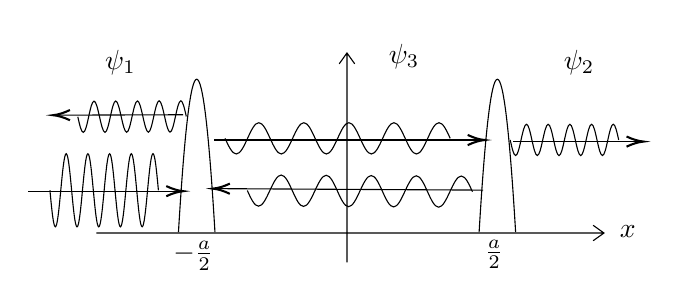
\begin{tikzpicture}[x=0.7pt,y=0.7pt,yscale=-0.8,xscale=0.8]
%uncomment if require: \path (0,310); %set diagram left start at 0, and has height of 310

%Shape: Axis 2D [id:dp004472866488251626] 
\draw  (172,188) -- (499.5,188)(333.66,71.83) -- (333.66,207) (492.5,183) -- (499.5,188) -- (492.5,193) (328.66,78.83) -- (333.66,71.83) -- (338.66,78.83)  ;
%Shape: Parabola [id:dp11125944654383879] 
\draw   (248.49,187.43) .. controls (240.64,55.86) and (232.79,55.86) .. (224.94,187.43) ;
%Shape: Wave [id:dp436578555794244] 
\draw   (142,160.42) .. controls (143.14,172.5) and (144.23,184) .. (145.5,184) .. controls (146.77,184) and (147.86,172.5) .. (149,160.42) .. controls (150.14,148.34) and (151.23,136.83) .. (152.5,136.83) .. controls (153.77,136.83) and (154.86,148.34) .. (156,160.42) .. controls (157.14,172.5) and (158.23,184) .. (159.5,184) .. controls (160.77,184) and (161.86,172.5) .. (163,160.42) .. controls (164.14,148.34) and (165.23,136.83) .. (166.5,136.83) .. controls (167.77,136.83) and (168.86,148.34) .. (170,160.42) .. controls (171.14,172.5) and (172.23,184) .. (173.5,184) .. controls (174.77,184) and (175.86,172.5) .. (177,160.42) .. controls (178.14,148.34) and (179.23,136.83) .. (180.5,136.83) .. controls (181.77,136.83) and (182.86,148.34) .. (184,160.42) .. controls (185.14,172.5) and (186.23,184) .. (187.5,184) .. controls (188.77,184) and (189.86,172.5) .. (191,160.42) .. controls (192.14,148.34) and (193.23,136.83) .. (194.5,136.83) .. controls (195.77,136.83) and (196.86,148.34) .. (198,160.42) .. controls (199.14,172.5) and (200.23,184) .. (201.5,184) .. controls (202.77,184) and (203.86,172.5) .. (205,160.42) .. controls (206.14,148.34) and (207.23,136.83) .. (208.5,136.83) .. controls (209.77,136.83) and (210.86,148.34) .. (212,160.42) ;
%Straight Lines [id:da9633291758111475] 
\draw    (128,161) -- (226,161) ;
\draw [shift={(228,161)}, rotate = 180] [color={rgb, 255:red, 0; green, 0; blue, 0 }  ][line width=0.75]    (10.93,-3.29) .. controls (6.95,-1.4) and (3.31,-0.3) .. (0,0) .. controls (3.31,0.3) and (6.95,1.4) .. (10.93,3.29)   ;
%Shape: Wave [id:dp07292774106378697] 
\draw   (255,126.92) .. controls (257.37,132.08) and (259.64,137) .. (262.26,137) .. controls (264.89,137) and (267.16,132.08) .. (269.53,126.92) .. controls (271.9,121.75) and (274.16,116.83) .. (276.79,116.83) .. controls (279.42,116.83) and (281.69,121.75) .. (284.06,126.92) .. controls (286.43,132.08) and (288.69,137) .. (291.32,137) .. controls (293.95,137) and (296.22,132.08) .. (298.59,126.92) .. controls (300.96,121.75) and (303.22,116.83) .. (305.85,116.83) .. controls (308.48,116.83) and (310.75,121.75) .. (313.12,126.92) .. controls (315.49,132.08) and (317.75,137) .. (320.38,137) .. controls (323.01,137) and (325.28,132.08) .. (327.65,126.92) .. controls (330.01,121.75) and (332.28,116.83) .. (334.91,116.83) .. controls (337.54,116.83) and (339.81,121.75) .. (342.17,126.92) .. controls (344.54,132.08) and (346.81,137) .. (349.44,137) .. controls (352.07,137) and (354.33,132.08) .. (356.7,126.92) .. controls (359.07,121.75) and (361.34,116.83) .. (363.97,116.83) .. controls (366.6,116.83) and (368.86,121.75) .. (371.23,126.92) .. controls (373.6,132.08) and (375.87,137) .. (378.5,137) .. controls (381.13,137) and (383.39,132.08) .. (385.76,126.92) .. controls (388.13,121.75) and (390.4,116.83) .. (393.03,116.83) .. controls (395.66,116.83) and (397.92,121.75) .. (400.29,126.92) ;
%Straight Lines [id:da2462983431835949] 
\draw    (248.15,128) -- (420.5,128) ;
\draw [shift={(422.5,128)}, rotate = 180] [color={rgb, 255:red, 0; green, 0; blue, 0 }  ][line width=0.75]    (10.93,-3.29) .. controls (6.95,-1.4) and (3.31,-0.3) .. (0,0) .. controls (3.31,0.3) and (6.95,1.4) .. (10.93,3.29)   ;
%Shape: Wave [id:dp44046816008414436] 
\draw   (229.99,112.77) .. controls (228.83,107.61) and (227.72,102.69) .. (226.46,102.7) .. controls (225.19,102.7) and (224.12,107.62) .. (222.99,112.79) .. controls (221.87,117.96) and (220.79,122.88) .. (219.52,122.89) .. controls (218.26,122.89) and (217.15,117.98) .. (215.99,112.82) .. controls (214.83,107.65) and (213.72,102.74) .. (212.46,102.74) .. controls (211.19,102.75) and (210.12,107.67) .. (208.99,112.84) .. controls (207.87,118.01) and (206.79,122.93) .. (205.52,122.93) .. controls (204.26,122.94) and (203.15,118.02) .. (201.99,112.86) .. controls (200.83,107.7) and (199.72,102.79) .. (198.46,102.79) .. controls (197.19,102.79) and (196.12,107.72) .. (194.99,112.89) .. controls (193.87,118.05) and (192.79,122.98) .. (191.52,122.98) .. controls (190.26,122.98) and (189.15,118.07) .. (187.99,112.91) .. controls (186.83,107.75) and (185.72,102.83) .. (184.46,102.84) .. controls (183.19,102.84) and (182.12,107.76) .. (180.99,112.93) .. controls (179.87,118.1) and (178.79,123.02) .. (177.52,123.03) .. controls (176.26,123.03) and (175.15,118.12) .. (173.99,112.95) .. controls (172.83,107.79) and (171.72,102.88) .. (170.46,102.88) .. controls (169.19,102.89) and (168.12,107.81) .. (166.99,112.98) .. controls (165.87,118.15) and (164.79,123.07) .. (163.52,123.07) .. controls (162.26,123.08) and (161.15,118.16) .. (159.99,113) .. controls (159.99,113) and (159.99,113) .. (159.99,113) ;
%Straight Lines [id:da8804045752381847] 
\draw    (227.99,111.69) -- (145.99,111.96) ;
\draw [shift={(143.99,111.97)}, rotate = 359.81] [color={rgb, 255:red, 0; green, 0; blue, 0 }  ][line width=0.75]    (10.93,-3.29) .. controls (6.95,-1.4) and (3.31,-0.3) .. (0,0) .. controls (3.31,0.3) and (6.95,1.4) .. (10.93,3.29)   ;
%Shape: Parabola [id:dp8087868429210319] 
\draw   (442.49,187.43) .. controls (434.64,55.86) and (426.79,55.86) .. (418.94,187.43) ;
%Shape: Wave [id:dp6830193103316252] 
\draw   (439,127.92) .. controls (440.14,133.08) and (441.23,138) .. (442.5,138) .. controls (443.77,138) and (444.86,133.08) .. (446,127.92) .. controls (447.14,122.75) and (448.23,117.83) .. (449.5,117.83) .. controls (450.77,117.83) and (451.86,122.75) .. (453,127.92) .. controls (454.14,133.08) and (455.23,138) .. (456.5,138) .. controls (457.77,138) and (458.86,133.08) .. (460,127.92) .. controls (461.14,122.75) and (462.23,117.83) .. (463.5,117.83) .. controls (464.77,117.83) and (465.86,122.75) .. (467,127.92) .. controls (468.14,133.08) and (469.23,138) .. (470.5,138) .. controls (471.77,138) and (472.86,133.08) .. (474,127.92) .. controls (475.14,122.75) and (476.23,117.83) .. (477.5,117.83) .. controls (478.77,117.83) and (479.86,122.75) .. (481,127.92) .. controls (482.14,133.08) and (483.23,138) .. (484.5,138) .. controls (485.77,138) and (486.86,133.08) .. (488,127.92) .. controls (489.14,122.75) and (490.23,117.83) .. (491.5,117.83) .. controls (492.77,117.83) and (493.86,122.75) .. (495,127.92) .. controls (496.14,133.08) and (497.23,138) .. (498.5,138) .. controls (499.77,138) and (500.86,133.08) .. (502,127.92) .. controls (503.14,122.75) and (504.23,117.83) .. (505.5,117.83) .. controls (506.77,117.83) and (507.86,122.75) .. (509,127.92) ;
%Straight Lines [id:da3372080950026667] 
\draw    (441,129) -- (523,129) ;
\draw [shift={(525,129)}, rotate = 180] [color={rgb, 255:red, 0; green, 0; blue, 0 }  ][line width=0.75]    (10.93,-3.29) .. controls (6.95,-1.4) and (3.31,-0.3) .. (0,0) .. controls (3.31,0.3) and (6.95,1.4) .. (10.93,3.29)   ;
%Shape: Wave [id:dp18490701651280472] 
\draw   (414.65,161.37) .. controls (412.31,156.19) and (410.07,151.26) .. (407.44,151.24) .. controls (404.81,151.23) and (402.52,156.13) .. (400.12,161.28) .. controls (397.72,166.44) and (395.43,171.34) .. (392.8,171.33) .. controls (390.17,171.31) and (387.93,166.38) .. (385.59,161.2) .. controls (383.25,156.02) and (381.01,151.09) .. (378.38,151.08) .. controls (375.76,151.06) and (373.46,155.97) .. (371.06,161.12) .. controls (368.67,166.27) and (366.37,171.18) .. (363.74,171.16) .. controls (361.11,171.15) and (358.87,166.22) .. (356.53,161.04) .. controls (354.19,155.86) and (351.96,150.93) .. (349.33,150.92) .. controls (346.7,150.9) and (344.4,155.81) .. (342.01,160.96) .. controls (339.61,166.11) and (337.31,171.02) .. (334.68,171) .. controls (332.06,170.99) and (329.82,166.06) .. (327.48,160.88) .. controls (325.14,155.7) and (322.9,150.77) .. (320.27,150.75) .. controls (317.64,150.74) and (315.35,155.65) .. (312.95,160.8) .. controls (310.55,165.95) and (308.26,170.85) .. (305.63,170.84) .. controls (303,170.83) and (300.76,165.89) .. (298.42,160.72) .. controls (296.08,155.54) and (293.84,150.61) .. (291.21,150.59) .. controls (288.58,150.58) and (286.29,155.48) .. (283.89,160.63) .. controls (281.49,165.79) and (279.2,170.69) .. (276.57,170.68) .. controls (273.94,170.66) and (271.7,165.73) .. (269.36,160.55) ;
%Straight Lines [id:da3169057197062486] 
\draw    (421.5,160.32) -- (249.16,159.36) ;
\draw [shift={(247.16,159.35)}, rotate = 0.32] [color={rgb, 255:red, 0; green, 0; blue, 0 }  ][line width=0.75]    (10.93,-3.29) .. controls (6.95,-1.4) and (3.31,-0.3) .. (0,0) .. controls (3.31,0.3) and (6.95,1.4) .. (10.93,3.29)   ;

% Text Node
\draw (508,181.4) node [anchor=north west][inner sep=0.75pt]    {$x$};
% Text Node
\draw (420.94,190.83) node [anchor=north west][inner sep=0.75pt]    {$\frac{a}{2}$};
% Text Node
\draw (219.94,191.83) node [anchor=north west][inner sep=0.75pt]    {$-\frac{a}{2}$};
% Text Node
\draw (176,68.4) node [anchor=north west][inner sep=0.75pt]    {$\psi _{1}$};
% Text Node
\draw (472,68.4) node [anchor=north west][inner sep=0.75pt]    {$\psi _{2}$};
% Text Node
\draw (359,64.4) node [anchor=north west][inner sep=0.75pt]    {$\psi _{3}$};

\end{tikzpicture}
\end{center}
Since the wavefunction is continuous,
\begin{equation}
    \psi_1\left(-\frac{a}{2}\right)=\psi_3\left(-\frac{a}{2}\right), \psi_3\left(\frac{a}{2}\right)=\psi_2\left(\frac{a}{2}\right).
\end{equation}
Thus,
\begin{equation}
    e^{-ik\frac{a}{2}}+Re^{ik\frac{a}{2}}=Ae^{-ik\frac{a}{2}}+Be^{ik\frac{a}{2}},
\end{equation}
\begin{equation}
    Se^{ik\frac{a}{2}}=Ae^{ik\frac{a}{2}}+Be^{-ik\frac{a}{2}}.
\end{equation}
Integrate the Schrödinger equation,
\begin{equation}
    \lim_{\epsilon\rightarrow0^+}\int_{x_0-\epsilon}^{x_0+\epsilon}\left[-\frac{\hbar^2}{2m}\frac{\dd^2}{\dd{x}^2}+V(x)\right]\psi(x)\dd{x}=\lim_{\epsilon\rightarrow0^+}\int_{x_0-\epsilon}^{x_0+\epsilon}E\psi(x)\dd{x}=0.
\end{equation}
i.e.
\begin{equation}
    \psi_3'\left(-\frac{a}{2}\right)-\psi'_1\left(-\frac{a}{2}\right)=\frac{2m\gamma}{\hbar^2}\psi\left(-\frac{a}{2}\right),
\end{equation}
\begin{equation}
    \psi_2'\left(\frac{a}{2}\right)-\psi'_3\left(\frac{a}{2}\right)=\frac{2m\gamma}{\hbar^2}\psi\left(\frac{a}{2}\right).
\end{equation}
Then we can deduce that,
\begin{eqnarray}
    A=\frac{2 (\sigma +2)}{\sigma ^2 \tau ^4-\sigma ^2+4},B=-\frac{2 \sigma  \tau
   ^2}{\sigma ^2 \tau ^4-\sigma ^2+4},\\
   R=-\frac{\left[(\sigma+1)^2-1\right](\tau^4-1)}{\tau ^2 \left(\sigma ^2 \tau ^4-\sigma ^2+4\right)},S=\frac{4}{\sigma ^2
   \tau ^4-\sigma ^2+4}
\end{eqnarray}
where
\begin{equation}
    \tau=e^{ik\frac{a}{2}},\ \sigma=\frac{2m\gamma}{ik\hbar^2}.
\end{equation}
When, $\left|S\right|=1$, $\tau^4=e^{i2ka}=1$, hence,
\begin{equation}
   \boxed{ ka=n\pi, \ n=1,2,3,\dots}
\end{equation}
(3) For bounded state, $\displaystyle\lim_{x\rightarrow-\infty}\mathrm{exp}(-ikx)=0$
\begin{equation}
    k=i\kappa=i\sqrt{-\frac{2mE}{\hbar^2}}.
\end{equation}
Let $\psi_1=Ce^{\kappa x},\psi_2=Ae^{\kappa x}\pm Ae^{-\kappa x},\psi_3=\pm Ce^{-\kappa x}$.\footnote{We set the odd or even parity solution.} Then,
\begin{equation}
    C\tau=A\tau\pm\frac{A}{\tau},
\end{equation}
\begin{equation}
    \left[C\tau-\left(A\tau \mp\frac{A}{\tau}\right)\right]=-\sigma C\tau.
\end{equation}
So,
\begin{equation}
    \sigma=\frac{2}{\pm\tau^2-1}.
\end{equation}
That's exactly the condition to make the denominator of $S$ and $R$ equal to $0$. That means the bounded state do not allow the wavefunction to have the form $\mathrm{exp}(-ikx)$.
\end{problem}
\begin{problem}[Bound states]
First, we clarify that if $V_1(x)<V_2(x),\ -\infty<x<+\infty$, then $E_{g1}<E_{g2}$. 
\begin{align}
    E_{g2}\ket{\psi_{g2}}=&\sum_{n}H_2\ket{\psi_{n1}}\braket{\psi_{n1}}{\psi_{g2}}\\
    =&\sum_{n}\left[H_1+(V_2-V_1)\right]\ket{\psi_{n1}}\braket{\psi_{n1}}{\psi_{g2}}\\
    =&\sum_{n}E_{n1}\ket{\psi_{g1}}\braket{\psi_{g1}}{\psi_{g2}}+(V_2-V_1)\ket{\psi_{g2}}\\
    \ge&E_{g1}\ket{\psi_{g2}}+(V_2-V_1)\ket{\psi_{g2}}
\end{align}
Thus,
\begin{equation}
    \left(E_{g1}-E_{g2}\right)\ket{\psi_{g2}}\le \int_{-\infty}^{+\infty}(V_1-V_2)\ket{x}\braket{x}{\psi_{g2}}\dd{x}<0\ket{\psi_{g2}}.
\end{equation}
\begin{equation}
    \boxed{E_{g1}<E_{g2}}
\end{equation}
Now,  let $V_2(x)=0$, then,
\begin{equation}
    \psi_2(x)=Ae^{-ikx}+Be^{ikx},
\end{equation}
where,
\begin{equation}
    k=\sqrt{\frac{2mE}{\hbar^2}}.
\end{equation}
If $E_{g2}<0$, then $k$ is an imaginary number. That contradicts to the finiteness of probability as $x\rightarrow\infty$. So $E_{g2}=0$. By the lemma, we obtain:
\begin{equation}
    \boxed{E_{g1}<0.}
\end{equation}
\end{problem}
\begin{problem}[Hermite Polynomial]
    (1) \begin{equation}
        \frac{\dd{u}}{\dd{z}}=\sum_{k=1}^{+\infty}ka_kz^{k-1}.
    \end{equation}
    \begin{equation}
        \frac{\dd^2 u}{\dd{z}^2}=\sum_{k=2}^{+\infty}k(k-1)a_kz^{k-2}.
    \end{equation}
    Then, 
    \begin{equation}
        \sum_{k=0}^{+\infty}\left[(k+2)(k+1)a_{k+2}-2ka_k+(\lambda_n-1)a_k\right]z^k=0.
    \end{equation}
    So, 
    \begin{equation}
        \frac{a_{k+2}}{a_k}=\frac{2k+1-\lambda_n}{(k+2)(k+1)}.
    \end{equation}
    $u_n$ is finite when $x\rightarrow\infty$, then there exists a $n$ such that $a_{n+2}=0$. We can deduce that
    \begin{equation}
        \boxed{\lambda_n=2n+1.}
    \end{equation}
    \begin{equation}
        E_n=\frac{1}{2}\lambda \hbar \omega=\left(n+\frac{1}{2}\right)\hbar\omega.
    \end{equation}
    (2) \begin{equation}
        e^{-(s-z)^2}=\sum_{n=0}^{\infty}\frac{H_n(z)e^{-z^2}}{n!}s^n.
    \end{equation}
    \begin{equation}
        H_n(z)e^{-z^2}=\left.\frac{\dd^n}{\dd{s}^n}e^{-(s-z)^2}\right|_{s=0}.
    \end{equation}
    $\dd{s}=-\dd{(z-s)}$, so 
    \begin{equation}
        \boxed{H_n(z)=(-)^ne^{z^2}\frac{\dd ^n}{\dd{z}^n}e^{-z^2}.}
    \end{equation}
    (3) \begin{equation}
        \frac{\pa G}{\pa s}=\sum_{n=0}^{\infty}\frac{1}{n!}H_{n+1}(z)s^n.
    \end{equation}
    \begin{equation}
        2sG=\sum_{n=1}^{\infty}2n\frac{1}{n!}H_{n-1}s^n.
    \end{equation}
    Compare the coefficients of $s^n$,
    \begin{equation}
        \boxed{H_{n+1}(z)-2zH_n(z)+2nH_{n-1}(z).}
    \end{equation}
    \begin{equation}
        \frac{\pa G}{\pa z}=\sum_{n=0}^{\infty}\frac{1}{n!}\frac{\dd}{\dd z}H_n(z)s^n.
    \end{equation}
    Hence,
    \begin{equation}
        \boxed{\frac{\dd}{\dd{z}}H_n=2nH_{n-1}.}
    \end{equation}
    (4) \begin{equation}
        \int_{-\infty}^{+\infty}G_1(s,z)G_2(t,z)\dd{z}=e^{-(z-(s+t))^2}e^{2st}=\Gamma(\frac{1}{2})e^{2st}.
    \end{equation}
    Therefore,
    \begin{equation}
        \boxed{ \int_{-\infty}^{+\infty}G_1(s,z)G_2(t,z)\dd{z}=\sqrt{\pi}e^{2st}.}
    \end{equation}
    \begin{equation}
        G_1(s,z)G_2(t,z)=\sum_{(n,m)\in \mathbb{N}^2}\frac{1}{n!m!}H_nH_ms^nt^m.
    \end{equation}
    \begin{equation}
        e^{2st}=\sum_{n=0}^{+\infty}\frac{(2st)^n}{n!}.
    \end{equation}
    Therefore,
    \begin{equation}
        \boxed{\int_{-\infty}^{+\infty}H_n(z)H_m(z)e^{-z^2}\dd{z}=\delta_{nm}2^nn!\sqrt{\pi}.}
    \end{equation}
\end{problem}
\end{document}